\section{Methodology}

We present an analytical and simulation models for coordination and distributed shared memory (DSM) architectures in warehouse graphs. The models compares centralized batch allocation with a DSM memory-agent approach, and derives propagation, claim, and queueing delay components to predict end-to-end order response times and stability conditions.

\begin{figure}[t]
  \centering
  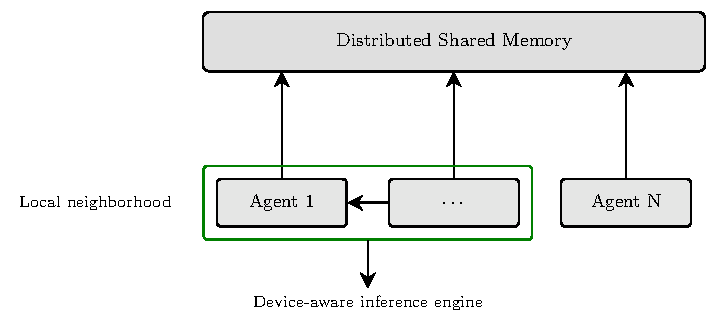
\includegraphics[width=\columnwidth]{../figures/dsm_architecture.pdf}
  \caption{High-level architecture: agents coordinate via a distributed shared memory fabric while running local device-aware inference.}
  \label{fig:dsm-arch}
\end{figure}
